%!TEX TS-program = xelatex
\documentclass{beamer}

\usepackage{HSE-theme/beamerthemeHSE-en} % Load HSE theme

%%% Fonts 
\usepackage{fontspec}
\defaultfontfeatures{Ligatures={TeX},Renderer=Basic}
\setmainfont[Ligatures={TeX,Historic}]{Myriad Pro} % install Myriad Pro or replace with Arial
\setsansfont{Myriad Pro}  % install Myriad Pro or replace with Arial
\setmonofont{Courier New}	

\usepackage{multicol} 		% Multiple columns
\graphicspath{{images/}}  	% Images folder

%%% Author and speech
\title[Short title]{Network Science} 
\subtitle{Project 1}
\author[Egor Dudyrev]{Egor Dudyrev \\ \smallskip \scriptsize \url{eodudyrev@edu.hse.ru}}
\institute[Higher School of Economics]{National Research University \\ Higher School of Economics (Moscow)}
\date{12.04.2020}

\begin{document}	% Document begins

\frame[plain]{\titlepage}	% Title frame

\section{Just some text}
\subsection{Subtitle}

\begin{frame}
\frametitle{Outline}
\begin{enumerate}
\item Network Summary
\begin{itemize}
\item Network Source
\item Network Layout
\item Network Characteristics
\end{itemize}
\item Structural Analysis
\begin{itemize}
\item Centrality measures
\item Page Rank
\item Assortative Mixing
\item Node structural equivalence
\item Closest random graph
\end{itemize}
\item Community Detection
\begin{itemize}
\item Clique search
\item Comminuty detection algorithms
\end{itemize}
\end{enumerate}

\end{frame}

\begin{frame}
\frametitle{Network Source}
The network is a graph of my friends and our mutual friends in VK social network.\\
\begin{multicols}{2}
\textbf{Properties}\\
\begin{itemize}
\item Order: 244 nodes
\item Size: 1657 edges
\end{itemize}
\columnbreak
\textbf{Node attributes}\\
\begin{itemize}
\item id
\item first name
\item last name
\item city
\item university name
\item faculty name
\end{itemize}
\end{multicols}
\end{frame}


\begin{frame}
\frametitle{Network Layout}
\begin{multicols}{2}
	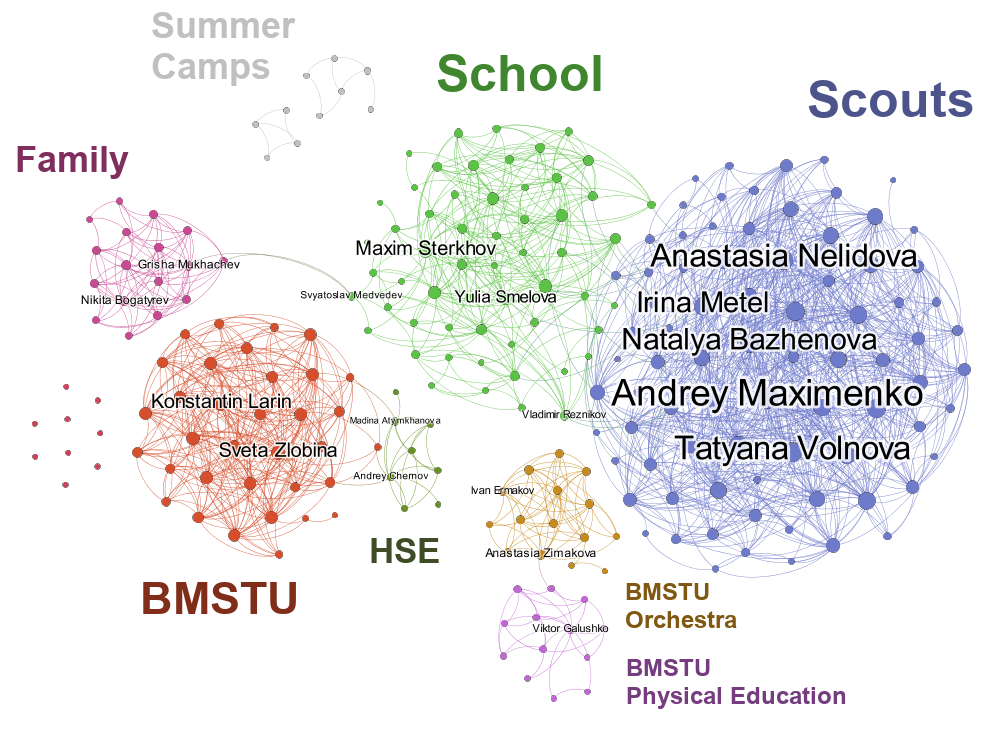
\includegraphics[width=\columnwidth]{Network_with_labels.png}
	\columnbreak

	Scouts are members of The Scout movements.\\
	\medskip
		Family, School and Scouts are mostly located in Udmurt republic. Other friends are mostly in Moscow.

\end{multicols}

\end{frame}

\begin{frame}
\frametitle{Network Characteristics}
\begin{multicols}{2}
	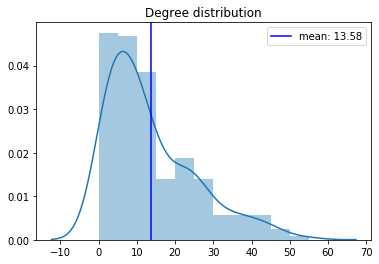
\includegraphics[width=\columnwidth]{Degree_distribution.png}
	\columnbreak

	\begin{itemize}
	\item Number of connected components: 14
	\item Diameters of connected components: 7, 5, 6, 3, 2, 0...
	\item Mean Clustering Coefficient: 0.5712
	\end{itemize}
\end{multicols}

\end{frame}


\begin{frame}
\frametitle{Centralities}
\begin{enumerate}
\item Degree Centrality
\item Closeness Centrality
\item Betweenness Centrality
\end{enumerate}

\end{frame}


\begin{frame}
\frametitle{Degree Centrality}
\begin{multicols}{2}
	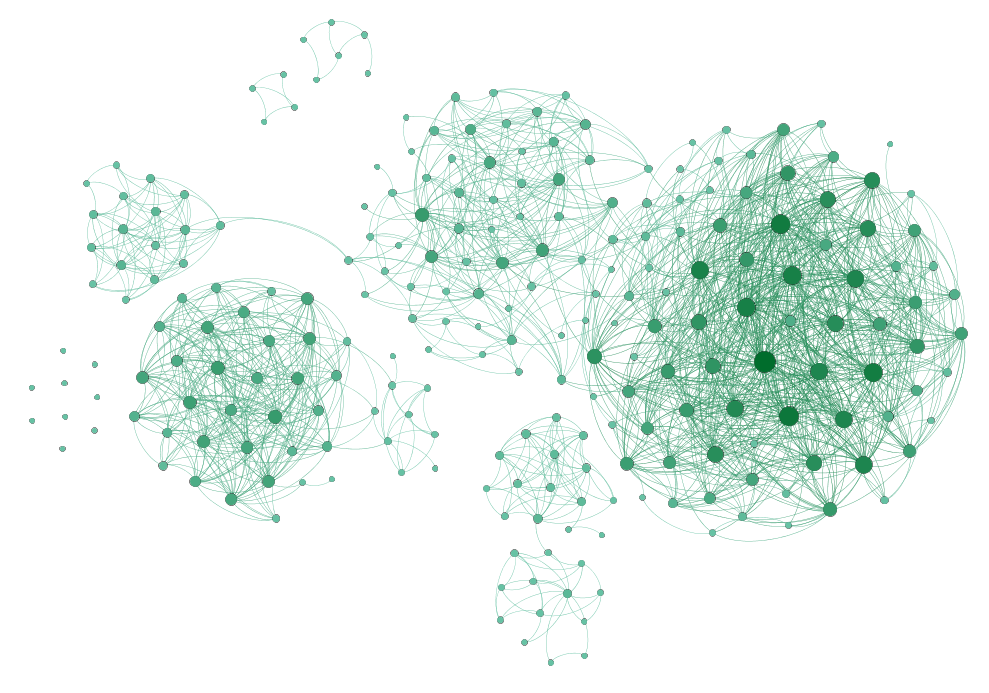
\includegraphics[width=\columnwidth]{Degree_centr.png}
	\columnbreak
	
	\textbf{Top nodes}
	\begin{enumerate}
	\item Andrey Maximenko:\\Formal and informal leader of Udmurtian Scouts\\(55 mutual friends)
	\item Tatyana Volnova:\\Formal leader of Udmurtian Scouts\\(49 mutual friends)
	\item Anastasia Nelidova:\\An experienced scout\\(47 mutual friends)
	\end{enumerate}
\end{multicols}

\end{frame}


\begin{frame}
\frametitle{Closeness Centrality}
\begin{multicols}{2}
	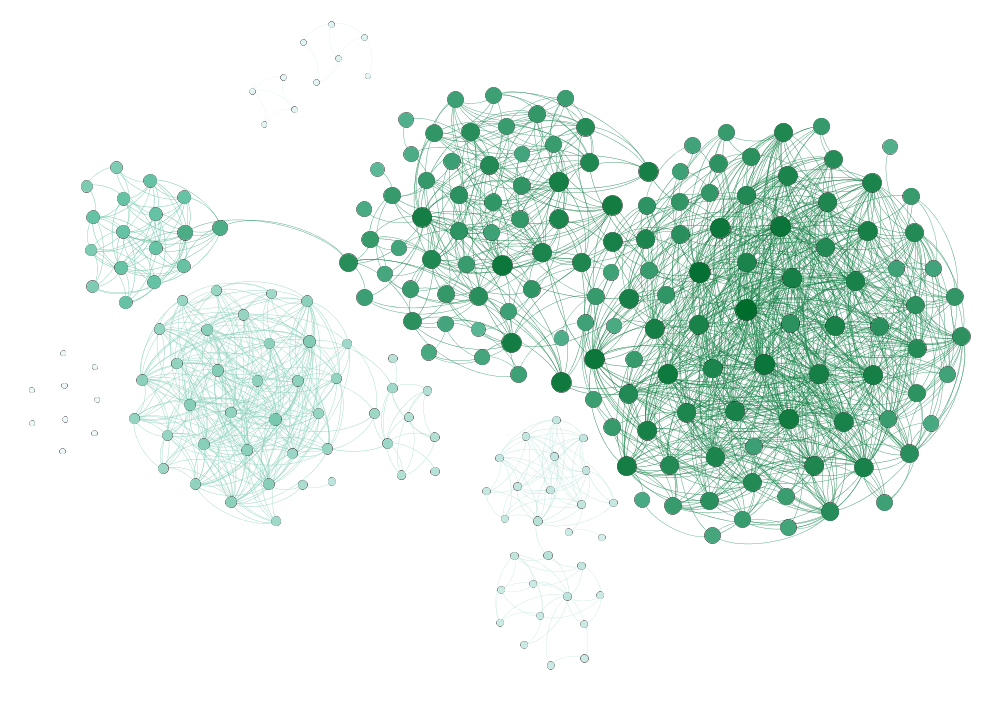
\includegraphics[width=\columnwidth]{Closeness_centr.png}
	\columnbreak
	
	\textbf{Top nodes}
	\begin{enumerate}
	\item Natalya Bazhenova:\\Formal leader of Udmurtian Scouts who now works in my school\\(avg. 2.18 handshakes)
	\item Irina "Metel":\\A scout leader who lives close to my school\\(avg. 2.23 handshakes)
	\item Anastasia Nelidova:\\An experienced scout\\(avg. 2.3 handshakes)
	\end{enumerate}
\end{multicols}

\end{frame}


\begin{frame}
\frametitle{Betweenness Centrality}
\begin{multicols}{2}
	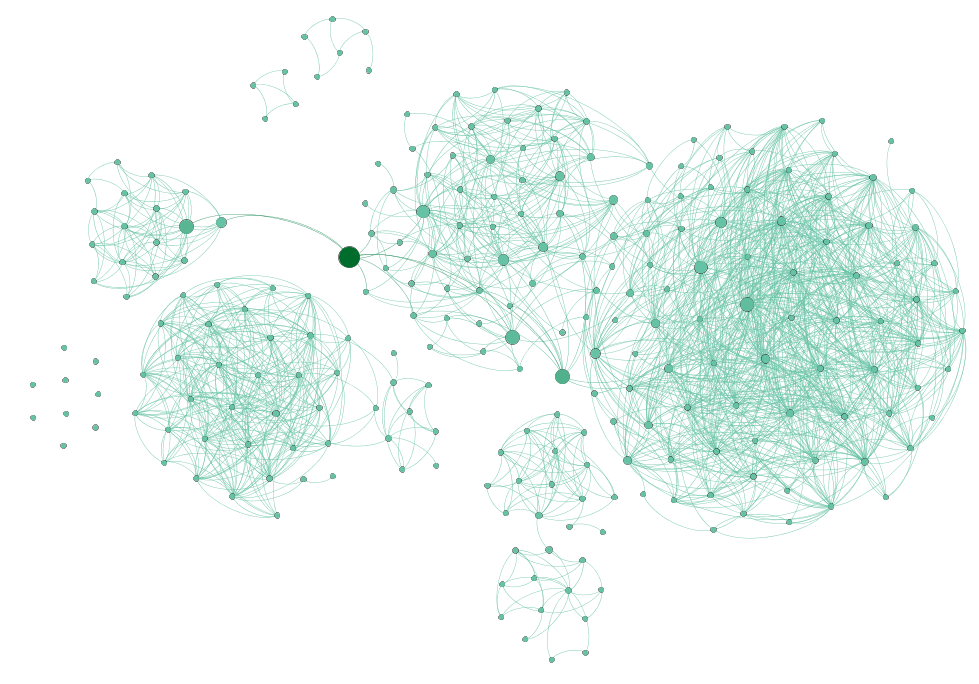
\includegraphics[width=\columnwidth]{Betweeness_centr.png}
	\columnbreak
	
	\textbf{Top nodes}
	\begin{enumerate}
	\item Svyatoslav Medvedev:\\Played in a school orchestra, knows some of my family\\(8\% smallest paths)
	\item Vladimir Reznikov:\\Played in a school orchestra, has a blog\\(4.8\% smallest paths)
	\item Grisha Mukhachev:\\Family, knows Svyatoslav Medvedev\\(4.5\% smallest paths)
	\end{enumerate}
\end{multicols}

\end{frame}


\begin{frame}
\frametitle{Page Rank}
\begin{multicols}{2}
	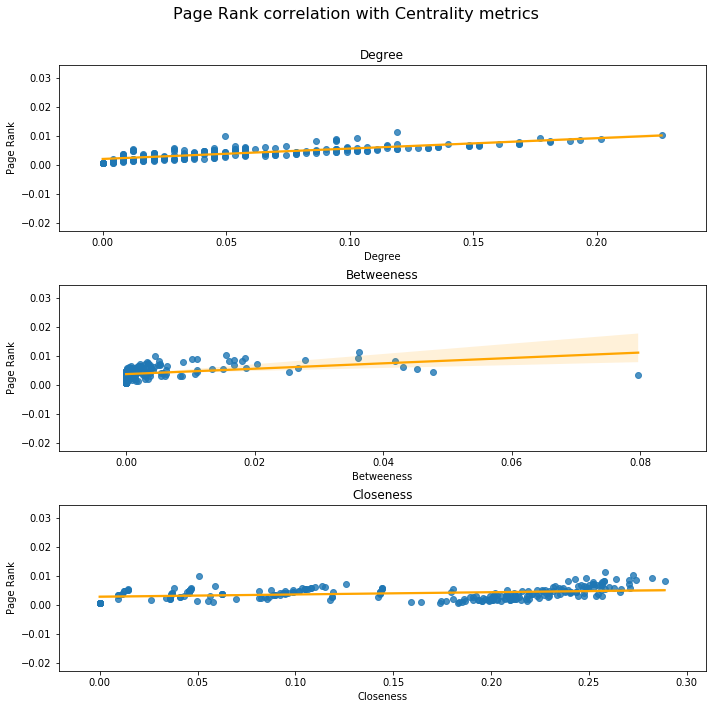
\includegraphics[width=\columnwidth]{page_rank_correlations.png}
	\columnbreak
	
	\textbf{Top nodes}
	\begin{enumerate}
	\item Maxim Sterkhov:\\Played in a school orchestra, knows some of my family\\(1.13\% smallest paths)
	\item Andrey Maximenko:\\Formal and informal Scout Leader\\(1.03\% smallest paths)
	\item Viktor Galushko:\\BMSTU PE teacher\\(1.01\% smallest paths)
	\end{enumerate}
\end{multicols}

\end{frame}

\begin{frame}
\frametitle{Assortative Mixing}
\begin{multicols}{2}
	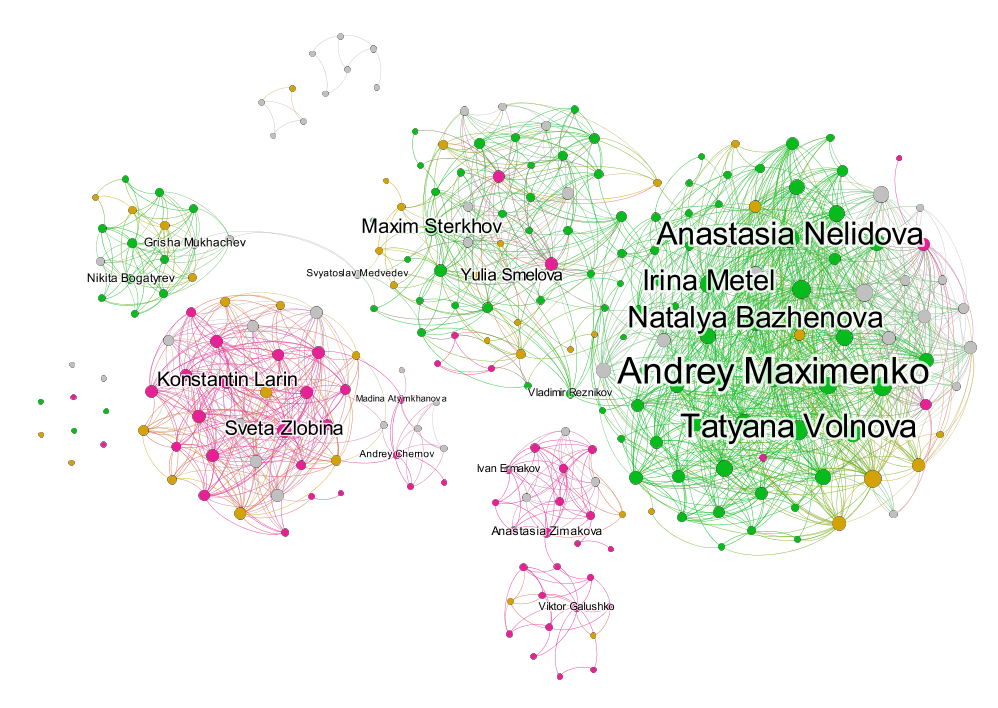
\includegraphics[width=\columnwidth]{nodes_by_city.png}
	\columnbreak
	
	\textbf{Assortativity Coefficients}
	\begin{enumerate}
	\item City: 0.21
	\item University: 0.1
	\item Faculty: 0.07
	\end{enumerate}
	\medskip	
	\textit{Colors}
	\begin{itemize}
	\item Green: Izhevsk
	\item Red: Moscow
	\item Orange: Saint-Petersburg
	\item Grey: Others
	\end{itemize}
	
\end{multicols}

\end{frame}


\begin{frame}
\frametitle{Node structural equivalence}
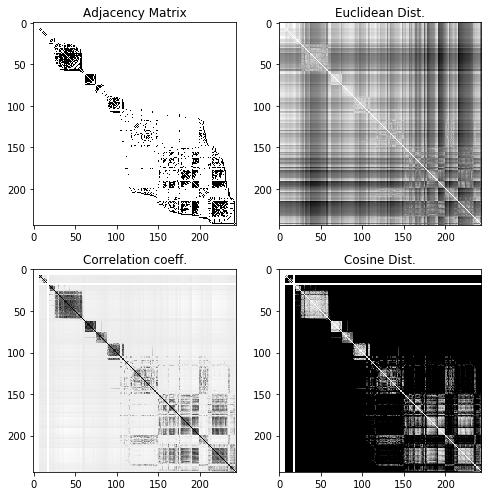
\includegraphics[width=0.5\textwidth]{node_structural_equivalence.png}
\end{frame}


\begin{frame}
\frametitle{Closest Random Graph model}
\begin{multicols}{2}
	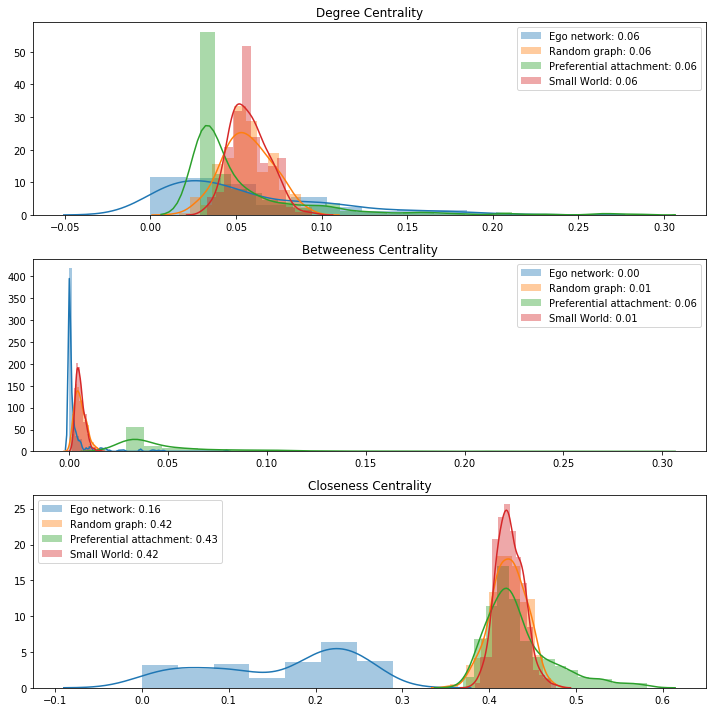
\includegraphics[width=\columnwidth]{random_graph.png}
	\columnbreak
	
	Comparing random graph models and Ego network centralities, we obtain ranks of the differences.\\
	\textbf{Mean difference rank}
	\begin{enumerate}
	\item Ego: 1
	\item Pref. attachment: 2.67
	\item Random graph: 3
	\item Small World: 3.33
	\end{enumerate}
	Therefore the closest random graph model in my case is Preferential attachemnt.
	
\end{multicols}

\end{frame}


\begin{frame}
\frametitle{Community Detection}
\begin{enumerate}
\item Clique Search
\item Community detection algorithms
\begin{itemize}
\item k-clique communities
\item Modularity based communities
\item Girvan-Newman
\end{itemize}
\end{enumerate}
\end{frame}


\begin{frame}
\frametitle{Clique search}
\begin{multicols}{2}
	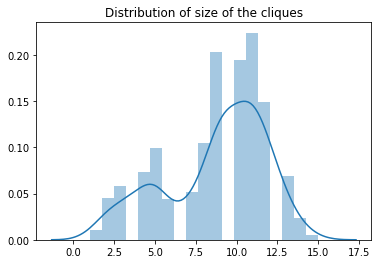
\includegraphics[width=\columnwidth]{clique_sizes.png}
	\columnbreak
	
	People are actively communicate in groups of 5 and 10 persons.\\This is totaly coherent with the basic theory of amount of people in small in medium size teams.
\end{multicols}

\end{frame}


\begin{frame}
\frametitle{k-clique communities}
\begin{multicols}{2}
	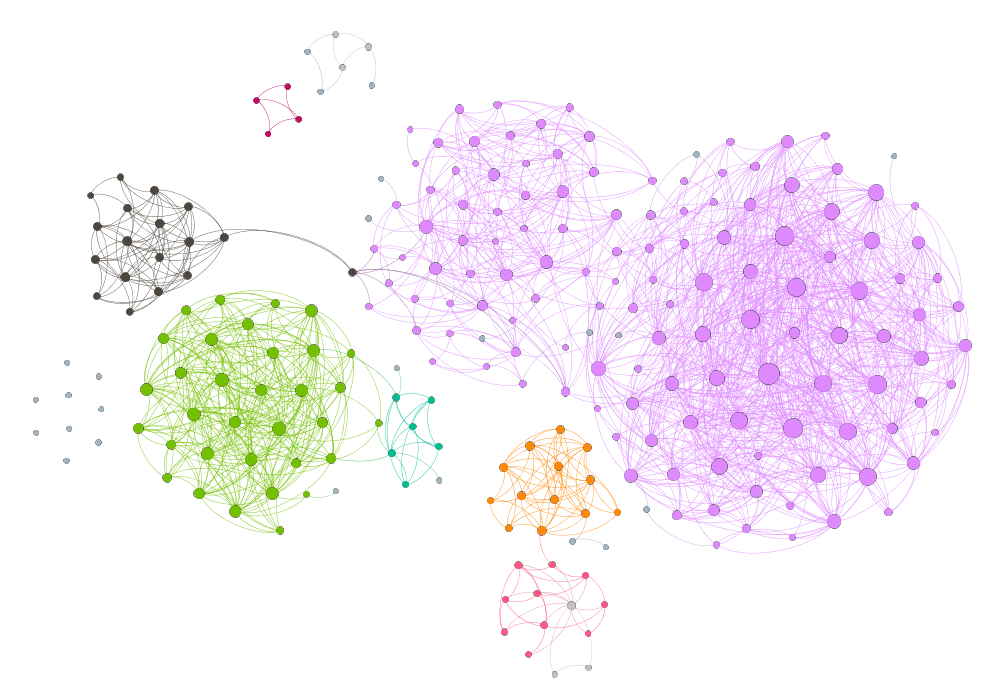
\includegraphics[width=\columnwidth]{kclique_comunity.png}
	\columnbreak
	
	Coefficient $k=3$\\
	\medskip
		Results are not well suited for the graph:
		\begin{itemize}
		\item Scouts and School communities are not splitted
		\item There are unclassified grey points in almost every community.
		\end{itemize}
\end{multicols}

\end{frame}

\begin{frame}
\frametitle{Modularity based communities}
\begin{multicols}{2}
	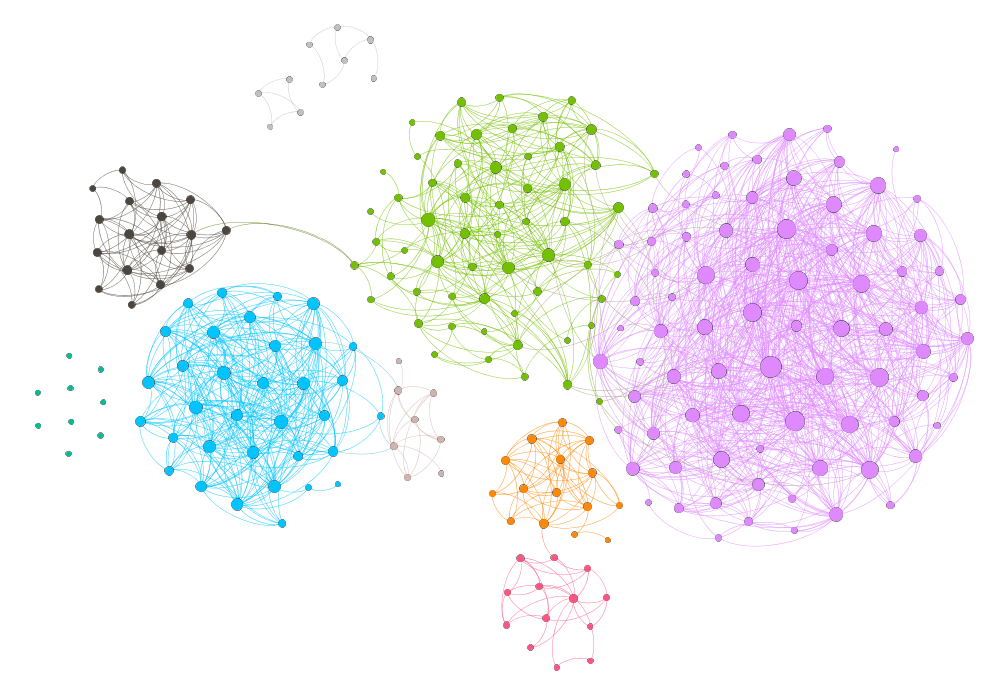
\includegraphics[width=\columnwidth]{modularity_based_comunity.png}
	\columnbreak
	
	The results perfectly lie on the network.
\end{multicols}

\end{frame}

\begin{frame}
\frametitle{Girvan-Newman communities}
\begin{multicols}{2}
	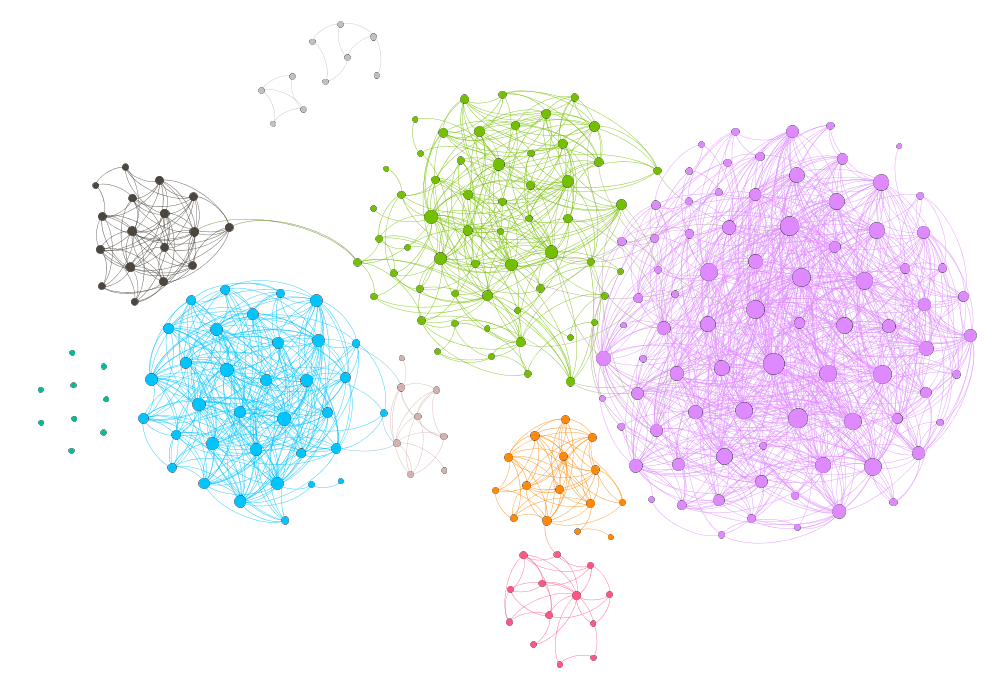
\includegraphics[width=\columnwidth]{girvan_newman_comunity.png}
	\columnbreak
	
	The results perfectly lie on the network.\\
	And they look much the same as Mularity based communities.\\
	\medskip
		These results were taken as ground truth and were shown in the very first network layout.
\end{multicols}

\end{frame}



\begin{frame}[c]
\begin{center}
\frametitle{\LARGE Thank you for your attention!}

{\LARGE \inserttitle}

\bigskip

{\insertauthor} 

\bigskip\bigskip

{\insertinstitute}

\bigskip\bigskip

{\large \insertdate}
\end{center}
\end{frame}

\end{document}